\documentclass[12pt, a4paper, oneside]{ctexart}
\usepackage{amsmath, amsthm, amssymb, bm, color, framed, graphicx, hyperref, mathrsfs, mathtools, enumerate, tikz}
\usepackage{float}
\usepackage{subcaption} 



\usetikzlibrary{patterns}

\title{\textbf{Homework 9}}
\author{萃英学院\qquad 2022级\qquad 王一鑫}
\date{\today}
\linespread{1.5}
\newcounter{problemname}
\newenvironment{problem}{\begin{framed}\stepcounter{problemname}\par\noindent\textsc{Problem \arabic{problemname}. }}{\end{framed}\par}
\newenvironment{solution}{%
	\par\noindent\textsc{Solution. }\ignorespaces
}{%
	\hfill$\qed$\par
}
\newenvironment{note}{\par\noindent\textsc{Note of Problem \arabic{problemname}. }}{\\\par}

\begin{document}
	
	\maketitle
	
	\begin{problem}
		(Exercise 5.2)

        Find the chromatic number of each graph in Fig \ref{fig:p1}.
        \begin{figure}[H]
            \small
            \centering
            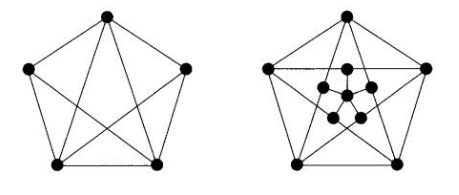
\includegraphics[width=0.8\columnwidth]{figure/fig1.png}
            \caption{Figure for Problem 1.}
            \label{fig:p1}
        \end{figure}
    
	\end{problem}
    
	\begin{solution}
       Apply Theorem 5.2. The largest vertex-degree of the left graph is $4$ and the right
       one is $5$. Thus the left graph is $4$-colourable and the right one is $5$-colourable.

       Moreover, the left graph is not $3$-colourable and the right one is not $4$-colourable.
       Thus the chromatic number of the left graph is $4$ and the right one is $5$.

		
	\end{solution}
		

		
	
	\begin{problem}
		(Exercise 5.6)

        A lecture timetable is to be drawn up. Since some students wish to attend several lectures, certain lectures must not coincide, as shown by asterisks in the following table. How many periods are needed to timetable all seven lectures?

        \begin{center}
        \begin{tabular}{c|ccccccc}
        & a & b & c & d & e & f & g \\
        \hline
        a & - & * & * & * & - & - & * \\
        b & * & - & * & * & * & - & * \\
        c & * & * & - & * & - & * & - \\
        d & * & * & * & - & - & * & - \\
        e & - & * & - & - & - & * & - \\
        f & - & - & * & * & - & - & * \\
        g & * & * & - & - & - & * & - \\
        \end{tabular}
        \end{center}

	\end{problem}
	
	\begin{solution}
		
		To answer this, we draw the graph whose vertices correspond to the seven lectures,
        with two vertices adjacent whenever te corresponding lectures are to be kept apart, see
        Fig \ref{fig:p2}. Now we colour the vertices, then the colours correspond to the periods
        needed, thus $4$ periods are needed.

        \begin{figure}[H]
            \small
            \centering
            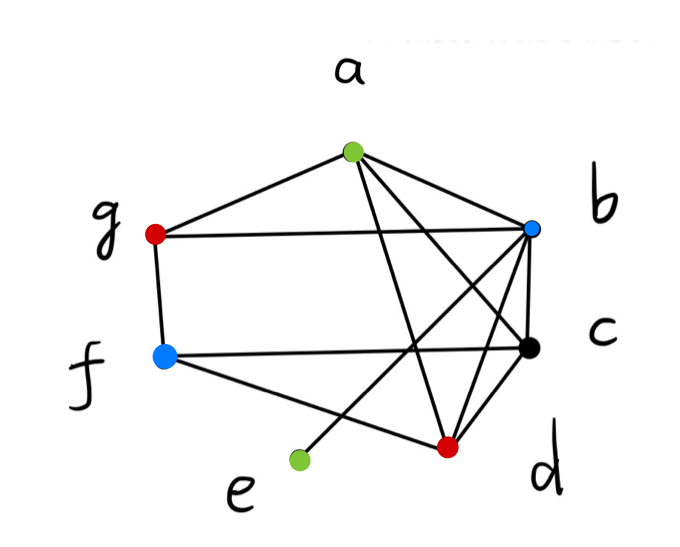
\includegraphics[width=0.35\columnwidth]{figure/fig2.PNG}
            \caption{Corresponding graph.}
            \label{fig:p2}
        \end{figure}
	\end{solution}
	
	\begin{problem}
        (Exercise 5.7)

        Let $G$ be a simple graph with $n$ vertices, which is regular of degree $d$. 
        By considering the number of vertices that can be assigned the same colour, 
        prove that $\chi(G) \geq \frac{n}{n - d}$.

	\end{problem}
	
	\begin{solution}
       
        If $c_i$ is the number of vertices coloured $i$, for $1 \leq i \leq \chi(G)$, then $c_i \leq n - d$. \\
        Thus, 
        \[
        n \leq c_1 + c_2 + \cdots + c_{\chi(G)} \leq \chi(G) \times (n - d),
        \]
        and so 
        \[
        \chi(G) \geq \frac{n}{n - d}.
        \]

	\end{solution}
	
	
	
	\begin{problem}
        (Exercise 5.8) 
        
        Let $G$ be a simple planar graph containing no triangles.
        \begin{itemize}
        \item[(i)] Using Euler's formula, show that $G$ contains a vertex of degree at most 3.
        \item[(ii)] Use induction to deduce that $G$ is 4-colourable.\\
        \textit{(In fact, it can be proved that $G$ is 3-colourable.)}
        \end{itemize}

	\end{problem}
	
	\begin{solution}
     
        \begin{itemize}
            \item[(i)] Without loss of generality we can assume that $G$ is connected
            and has at least three vertices. If each vertex has degree at least $4$, 
            then, with the above notation, we have
            \[
            4n \leq 2m, \text{ so } 2n \leq m.
            \]
            It follows immediately from Corollary 4.8(ii) that
            \[
            2n \leq 2n - 4,
            \]
            which is a contradiction. 
            \item[(ii)] We prove the theorem by induction on the number of vertices.
            Suppose then that $G$ is a simple planar graph with $n$ vertices, 
            and that all simple planar graphs with $n - 1$ vertices are 4-colourable. 
            By (i), $G$ contains a vertex $v$ of degree at most 3. 
            If we delete $v$ and its incident edges, then the graph that remains has 
            $n - 1$ vertices and is thus 4-colourable. A 4-colouring of $G$ 
            is then obtained by colouring $v$ with a colour different from the (at most three) 
            vertices adjacent to $v$.
            
        \end{itemize}
		
	\end{solution}


	\begin{problem}
		(Exercise 5.11)

        \begin{enumerate}
            \item[(i)] Find the chromatic polynomials of the six connected simple graphs on four vertices.
            \item[(ii)] Verify that each of the polynomials in part (i) has the form
            \[
            k^4 - mk^3 + ak^2 - bk,
            \]
            where $m$ is the number of edges, and $a$ and $b$ are positive constants.
          \end{enumerate}
          
        
    \end{problem}

	\begin{solution}
       All 6 graphs are shown in Fig 3.
        \begin{enumerate}[(i)]
            \item 
                \begin{figure}[htbp]
                \centering
                
                % 1. Path graph P4
                \begin{subfigure}{0.3\textwidth}
                \centering
                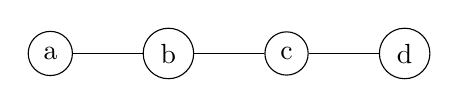
\begin{tikzpicture}[scale=1, every node/.style={circle, draw, fill=white}]
                \node (a) at (0,0) {a};
                \node (b) at (1.5,0) {b};
                \node (c) at (3,0) {c};
                \node (d) at (4.5,0) {d};
                \draw (a) -- (b) -- (c) -- (d);
                \end{tikzpicture}
                \caption{Path $P_4$}
                \end{subfigure}
                %
                % 2. Star K1,3
                \begin{subfigure}{0.3\textwidth}
                \centering
                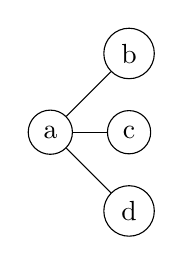
\begin{tikzpicture}[scale=1, every node/.style={circle, draw, fill=white}]
                \node (a) at (0,0) {a};
                \node (b) at (1,1) {b};
                \node (c) at (1,0) {c};
                \node (d) at (1,-1) {d};
                \draw (a) -- (b);
                \draw (a) -- (c);
                \draw (a) -- (d);
                \end{tikzpicture}
                \caption{Star $K_{1,3}$}
                \end{subfigure}
                %
                % 3. Cycle C4
                \begin{subfigure}{0.3\textwidth}
                \centering
                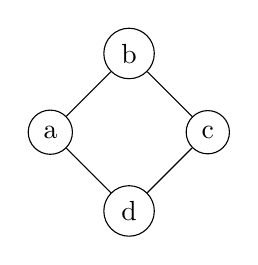
\begin{tikzpicture}[scale=1, every node/.style={circle, draw, fill=white}]
                \node (a) at (0,0) {a};
                \node (b) at (1,1) {b};
                \node (c) at (2,0) {c};
                \node (d) at (1,-1) {d};
                \draw (a) -- (b) -- (c) -- (d) -- (a);
                \end{tikzpicture}
                \caption{Cycle $C_4$}
                \end{subfigure}
                
                \vspace{1cm}
                
                % 4. Diamond (K4 minus edge)
                \begin{subfigure}{0.3\textwidth}
                \centering
                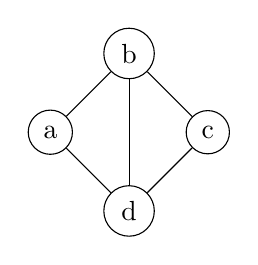
\begin{tikzpicture}[scale=1, every node/.style={circle, draw, fill=white}]
                \node (a) at (0,0) {a};
                \node (b) at (1,1) {b};
                \node (c) at (2,0) {c};
                \node (d) at (1,-1) {d};
                \draw (a) -- (b) -- (c) -- (d) -- (a);
                \draw (b) -- (d);
                \end{tikzpicture}
                \caption{Diamond}
                \end{subfigure}
                %
                % 5. Kite graph
                \begin{subfigure}{0.3\textwidth}
                \centering
                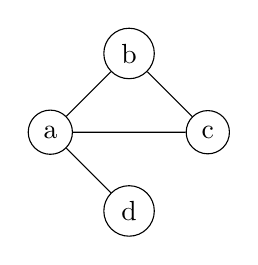
\begin{tikzpicture}[scale=1, every node/.style={circle, draw, fill=white}]
                \node (a) at (0,0) {a};
                \node (b) at (1,1) {b};
                \node (c) at (2,0) {c};
                \node (d) at (1,-1) {d};
                \draw (a) -- (b) -- (c) -- (a);
                \draw (a) -- (d);
                \end{tikzpicture}
                \caption{Kite graph}
                \end{subfigure}
                %
                % 6. Complete graph K4
                \begin{subfigure}{0.3\textwidth}
                \centering
                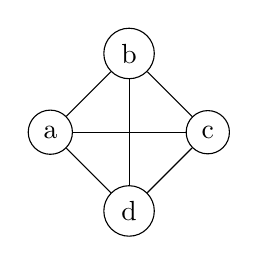
\begin{tikzpicture}[scale=1, every node/.style={circle, draw, fill=white}]
                \node (a) at (0,0) {a};
                \node (b) at (1,1) {b};
                \node (c) at (2,0) {c};
                \node (d) at (1,-1) {d};
                \draw (a) -- (b) -- (c) -- (d) -- (a);
                \draw (a) -- (c);
                \draw (b) -- (d);
                \end{tikzpicture}
                \caption{Complete graph $K_4$}
                \end{subfigure}
                \caption{All six connected simple graphs on four vertices}
                \end{figure}
                \begin{itemize}
                    \item \textbf{1. Path graph $P_4$:}
                    \[
                    P_{P_4}(k) = k(k - 1)^3
                    \]
                  
                    \item \textbf{2. Star graph $K_{1,3}$:}
                    \[
                    P_{K_{1,3}}(k) = k(k - 1)^3
                    \]
                  
                    \item \textbf{3. Cycle graph $C_4$:}
                    \[
                    P_{C_4}(k) = k(k - 1)^2(k - 2)
                    \]
                  
                    \item \textbf{4. Diamond graph (i.e., $K_4$ minus one edge):}
                    \[
                    P_{\text{diamond}}(k) = k(k - 1)(k - 2)^2
                    \]
                  
                    \item \textbf{5. Kite graph:}
                    \[
                    P_{\text{kite}}(k) = k(k - 1)^2(k - 2)
                    \]
                  
                    \item \textbf{6. Complete graph $K_4$:}
                    \[
                    P_{K_4}(k) = k(k - 1)(k - 2)(k - 3)
                    \]
                  \end{itemize}
            \item \begin{itemize}
                \item \textbf{1. Path graph $P_4$:}
                \[
                P_{P_4}(k) = k(k - 1)^3 = k^4 - 3k^3 + 3k^2 - k
                \]
              
                \item \textbf{2. Star graph $K_{1,3}$:}
                \[
                P_{K_{1,3}}(k) = k(k - 1)^3 = k^4 - 3k^3 + 3k^2 - k
                \]
              
                \item \textbf{3. Cycle graph $C_4$:}
                \[
                P_{C_4}(k) = k(k - 1)^2(k - 2) = k^4 - 4k^3 + 6k^2 - 3k
                \]
              
                \item \textbf{4. Diamond graph:}
                \[
                P_{\text{diamond}}(k) = k(k - 1)^2(k - 2) = k^4 - 5k^3 + 10k^2 - 8k
                \]
              
                \item \textbf{5. Kite graph:}
                \[
                P_{\text{kite}}(k) = k(k - 1)(k - 2)^2 = k^4 - 4k^3 + 5k^2 - 2k
                \]
              
                \item \textbf{6. Complete graph $K_4$:}
                \[
                P_{K_4}(k) = k(k - 1)(k - 2)(k - 3) = k^4 - 6k^3 + 11k^2 - 6k
                \]
              \end{itemize}
             So the polynomials in part (i) has the form
            \[
            k^4 - mk^3 + ak^2 - bk,
            \]
            where $m$ is the number of edges, and $a$ and $b$ are positive constants.
        \end{enumerate}
		

    \end{solution}
		
    
	\begin{problem}
		(Exercise 5.13)

		\begin{enumerate}
            \item[(i)] Prove that the chromatic polynomial of $K_{2,s}$ is
            \[
            k(k - 1)^s + k(k - 1)(k - 2)^s.
            \]
            
            \item[(ii)] Prove that the chromatic polynomial of $C_n$ is
            \[
            (k - 1)^n + (-1)^n(k - 1).
            \]
          \end{enumerate}
          
    \end{problem}

	\begin{solution}
       
        \begin{enumerate}[(i)]
            \item Let the two parts of $K_{2,s}$ be:
            \begin{itemize}
                \item Set $A = \{a_1, a_2\}$
                \item Set $B = \{b_1, b_2, \dots, b_s\}$
            \end{itemize}            
            We compute the number of proper $k$-colorings of $K_{2,s}$ by separating into two cases:
            
            \medskip
            
            \textbf{Case 1: $a_1$ and $a_2$ are assigned the same color.}
            
            There are:
            \begin{itemize}
                \item $k$ choices for the common color of $a_1$ and $a_2$;
                \item Each vertex in $B$ must then avoid this color: $(k - 1)^s$ total choices.
            \end{itemize}
            
            So this case contributes:
            \[
            k(k - 1)^s.
            \]
            
            \medskip
            
            \textbf{Case 2: $a_1$ and $a_2$ are assigned different colors.}
            
            There are:
            \begin{itemize}
                \item $k(k - 1)$ ways to assign different colors to $a_1$ and $a_2$;
                \item Each vertex in $B$ must avoid both of these colors: $(k - 2)^s$ total choices.
            \end{itemize}
            
            So this case contributes:
            \[
            k(k - 1)(k - 2)^s.
            \]
            
            \medskip
            
            \textbf{Therefore,}
            \[
            P_{K_{2,s}}(k) = k(k - 1)^s + k(k - 1)(k - 2)^s.
            \]
            \item Apply Theorem 5.6.
            \[
            P_G(k) = P_{G - e}(k) - P_{G / e}(k),
            \]
            
            Choose any edge $e$ of $C_n$. Then:
            \begin{itemize}
              \item $C_n - e$ becomes a path graph $P_n$.
              \item $C_n / e$ becomes another cycle, but with $n - 1$ vertices, i.e., $C_{n - 1}$.
            \end{itemize}
            
            Thus, applying the deletion–contraction formula to $C_n$, we have the recurrence:
            \[
            P_{C_n}(k) = P_{P_n}(k) - P_{C_{n - 1}}(k).
            \]
            
            We already know the chromatic polynomial of a path graph $P_n$ is:
            \[
            P_{P_n}(k) = k(k - 1)^{n - 1}.
            \]
            
            Therefore, the recurrence becomes:
            \[
            P_{C_n}(k) = k(k - 1)^{n - 1} - P_{C_{n - 1}}(k).
            \]
            and 
            \[
                P_{C_n}(k) = (k - 1)^n + (-1)^n(k - 1).
            \]
            satisfies the relation.


        \end{enumerate}
		
	\end{solution}


	\begin{problem}
		(Exercise 5.14)
        
		Prove that, if $G$ is a disconnected simple graph, then its chromatic 
        polynomial $P_G(k)$ is the product of the chromatic polynomials of its components. 
        What can you say about the degree of the lowest non-vanishing term?


	\end{problem}

	\begin{solution}

        If $G$ is disconnected, then its components $G_1, G_2, \dots, G_r$ are vertex-disjoint and have no edges 
        between them. This means that the colorings on different components are completely independent, 
        a coloring on one component has no impact on the valid colorings of the others.

        Therefore, to obtain a proper coloring of the entire graph $G$, we simply choose a proper coloring 
        for each component $G_i$ independently. The total number of proper colorings of $G$ is the product 
        of the number of proper colorings of each $G_i$. Thus,
        \[
        P_G(k) = P_{G_1}(k) \cdot P_{G_2}(k) \cdots P_{G_r}(k) = \prod_{i=1}^r P_{G_i}(k).
        \]
        
        Each chromatic polynomial $P_{G_i}(k)$ has lowest non-zero term of degree 1.
        Thus, for $G$ with $r$ connected components, the lowest non-zero term of the product polynomial $P_G(k)$
        has degree $r$, since the product of $r$ polynomials each having lowest degree term $k$ 
        will yield a term of $k^r$ as the lowest-degree nonzero term.
        

		
	\end{solution}
     

    \begin{problem}
        (Exercise 5.16)

        \begin{enumerate}
            \item[(i)] Use the results of Exercises 5.14 and 5.15 to prove that, if
            \[
            P_G(k) = k(k - 1)^n,
            \]
            then $G$ is a tree on $n$ vertices.
            
            \item[(ii)] Find three graphs with chromatic polynomial
            \[
            k^5 - 4k^4 + 6k^3 - 4k^2 + k.
            \]
          \end{enumerate}          
		
    \end{problem}
	
    \begin{solution} 
       
		\begin{enumerate}
            \item[(i)] Since
            \[
            k(k - 1)^{n - 1} = k^n - (n - 1)k^{n - 1} + \cdots + (-1)^{n - 1}k,
            \]
            and $G$ has $n$ vertices, $n - 1$ edges and one component,  
            it follows from Theorem 3.1(iii) that $G$ is a tree on $n$ vertices.
          
            \item[(ii)] Since $P_G(k) = k(k - 1)^4$, $G$ must be a tree on five vertices:
          
            \begin{center}
                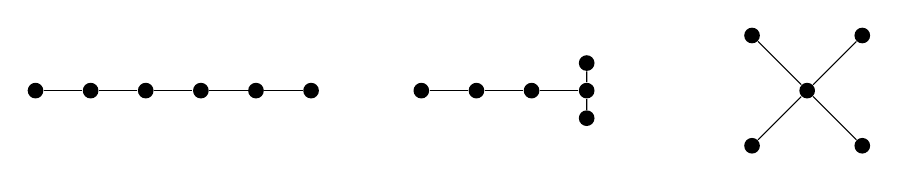
\begin{tikzpicture}[scale=0.7, every node/.style={circle, fill, inner sep=2pt}]
                    % 左侧线形图
                    \foreach \x in {0,...,5}
                        \node (a\x) at (\x,0) {};
                    \foreach \x in {0,...,4}
                        \draw (a\x) -- (a\the\numexpr\x+1\relax);
                    
                    % 中间“Y”型图
                    \foreach \x in {0,...,3}
                        \node (b\x) at (\x+7,0) {};
                    \node (b4) at (10,0.5) {};
                    \node (b5) at (10,-0.5) {};
                    \foreach \x in {0,...,2}
                        \draw (b\x) -- (b\the\numexpr\x+1\relax);
                    \draw (b3) -- (b4);
                    \draw (b3) -- (b5);
                    
                    % 右侧星型图
                    \node (c0) at (14,0) {};
                    \node (c1) at (13,1) {};
                    \node (c2) at (15,1) {};
                    \node (c3) at (13,-1) {};
                    \node (c4) at (15,-1) {};
                    \foreach \x in {1,2,3,4}
                        \draw (c0) -- (c\x);
                \end{tikzpicture}
                \end{center}
          \end{enumerate}
          
        
    \end{solution}

\end{document}


